\documentclass{paper}

%\usepackage{times}
\usepackage{epsfig}
\usepackage{graphicx}
\usepackage{amsmath}
\usepackage{amssymb}
\usepackage{color}
\usepackage{caption}
\usepackage{subcaption}


% load package with ``framed'' and ``numbered'' option.
%\usepackage[framed,numbered,autolinebreaks,useliterate]{mcode}

% something NOT relevant to the usage of the package.
\setlength{\parindent}{0pt}
\setlength{\parskip}{18pt}
\graphicspath{{images/}}


\usepackage[latin1]{inputenc} 
\usepackage[T1]{fontenc} 


\usepackage{listings} 
\lstset{% 
   language=Matlab, 
   basicstyle=\small\ttfamily, 
} 



\title{Final-Project}



\author{Jenni Simon\\09-116-005}
% //////////////////////////////////////////////////


\begin{document}



\maketitle


% Add figures:
%\begin{figure}[t]
%%\begin{center}
%\quad\quad   \includegraphics[width=1\linewidth]{ass2}
%%\end{center}
%
%\label{fig:performance}
%\end{figure}

\section*{Comparing heuristics for TSP}

\paragraph{1. Comparison based on achieved Loss values}

In this section, the implemented algorithms are compared based on the minimum, maximum and mean values of the loss-function achieved during $m=40$ runs. Tables \ref{tab:const}-\ref{tab:heatSA} summarise the results and also show 95\% confidence intervals for the true mean.


\begin{table}[!h]
\centering
\caption{Results for Construction Heuristics}
\label{tab:const}
\begin{tabular}{| l ||c|c|c|c|}
\hline
                       &  min & max & mean & 95\% confidence interval \\ \hline \hline
Best-Insertion &      1.4813   &      1.6081    &      1.5245     &      [1.5159,   1.5330]     \\  \hline 
Shortest-Edge  &    1.6197   &      1.7413    &      1.6725     &      [1.6638,   1.6813]      \\ \hline
Saving         &         1.7511   &      2.0129    &      1.8636     &      [1.8425,   1.8848]      \\ \hline
\end{tabular}
\end{table}

\begin{table}[!h]
\centering
\caption{Results for Greedy Local Search}
\label{tab:GLS}
\begin{tabular}{| l ||c|c|c|c|}
\hline
Move                  &  min & max & mean & 95\% confidence interval \\ \hline \hline
Swap              &      3.5400   &      4.2071    &      3.8952     &      [3.8384,   3.9521]     \\  \hline 
Translation       &    1.9867   &      2.5519    &      2.2730     &      [2.2332,   2.3128]      \\ \hline
Inversion     &         1.5052   &      1.6109    &      1.5512     &      [1.5421,   1.5604]      \\ \hline
Mixed          &         1.4664   &      1.5612    &      1.5055     &      [1.4982,   1.5127]      \\ \hline
\end{tabular}
\end{table}

\begin{table}[!h]
\centering
\caption{Results for Metropolis Simulated Annealing}
\label{tab:metroSA}
\begin{tabular}{| l ||c|c|c|c|}
\hline
Move                  &  min & max & mean & 95\% confidence interval \\ \hline \hline
Swap              &      3.2364   &      3.8152    &      3.5222     &      [3.4763,   3.5680]     \\  \hline 
Translation       &    1.9680   &      2.3782    &      2.1724     &      [2.1452,   2.1996]      \\ \hline
Inversion     &         1.4910   &      1.6040    &      1.5425     &      [1.5338,   1.5511]      \\ \hline
Mixed          &         1.4610   &      1.5689    &      1.5155     &      [1.5074,   1.5236]      \\ \hline
\end{tabular}
\end{table}

\begin{table}[!h]
\centering
\caption{Results for Heatbath Simulated Annealing}
\label{tab:heatSA}
\begin{tabular}{| l ||c|c|c|c|}
\hline
Move                  &  min & max & mean & 95\% confidence interval \\ \hline \hline
Swap              &      3.2542   &      4.3422    &      3.6040     &      [3.5380,   3.6701]     \\  \hline 
Translation       &    1.8958   &      2.4291    &      2.1767     &      [2.1390,   2.2144]      \\ \hline
Inversion     &         1.4937   &      1.5906    &      1.5417     &      [1.5340,   1.5493]      \\ \hline
Mixed          &         1.4723   &      1.5665    &      1.5192     &      [1.5116,   1.5267]      \\ \hline
\end{tabular}
\end{table}


\paragraph{2. Solution Paths}

This section provides figures of the best solution-paths per algorithm achieved after the $m=40$ runs. Figures \ref{fig:ConsPath}-\ref{fig:MixedPath} show the obtained paths. Note that they are not closed, making it possible to observe the starting point.

\begin{figure*}[!h]
    \makebox[\textwidth][c]{
    \begin{subfigure}[]{0.7\textwidth}
        \centering
        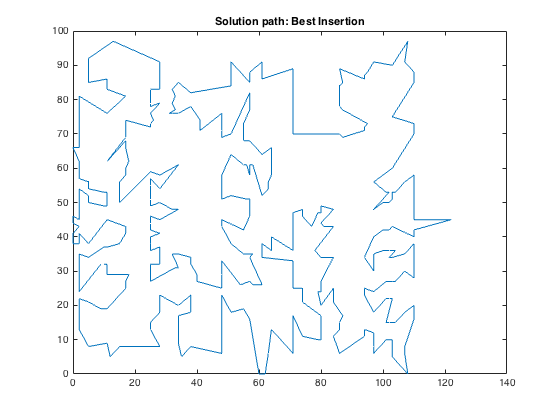
\includegraphics[width=\linewidth]{BestInsert_path}
    \end{subfigure}
    \begin{subfigure}[]{0.7\textwidth}
        \centering
        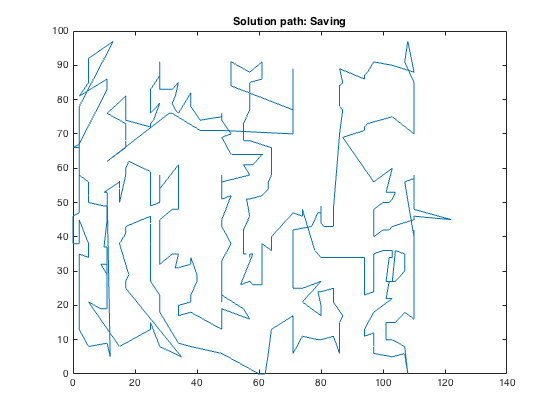
\includegraphics[width=\linewidth]{Saving_path}
    \end{subfigure}
    }
    \begin{subfigure}[]{\textwidth}
        \centering
        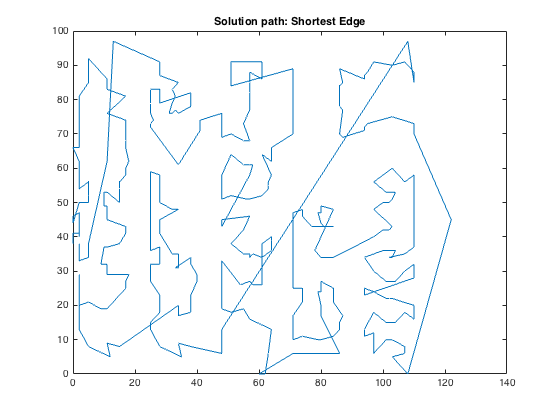
\includegraphics[width=0.7\linewidth]{ShortestEdge_path}
    \end{subfigure}
    \caption{Construction Heuristics}    
\label{fig:ConsPath}
\end{figure*}

\begin{figure*}[!h]
    \makebox[\textwidth][c]{
    \begin{subfigure}[]{0.7\textwidth}
        \centering
        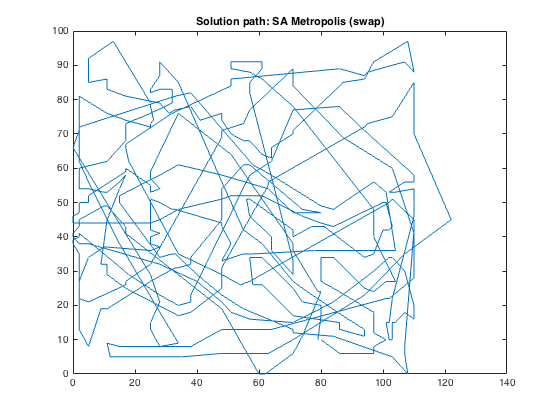
\includegraphics[width=\linewidth]{SAMetropolis(swap)}
    \end{subfigure}
    \begin{subfigure}[]{0.7\textwidth}
        \centering
        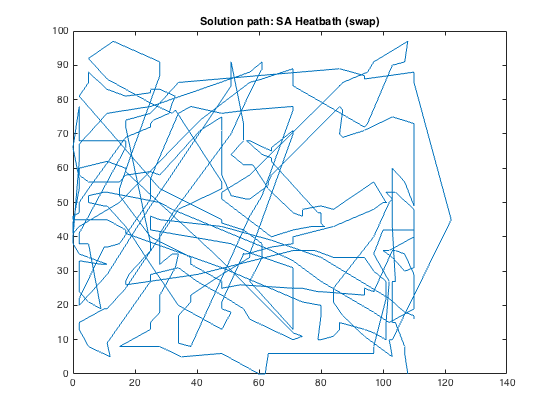
\includegraphics[width=\linewidth]{SAHeatbath(swap)}
    \end{subfigure}
    }
    \begin{subfigure}[]{\textwidth}
        \centering
        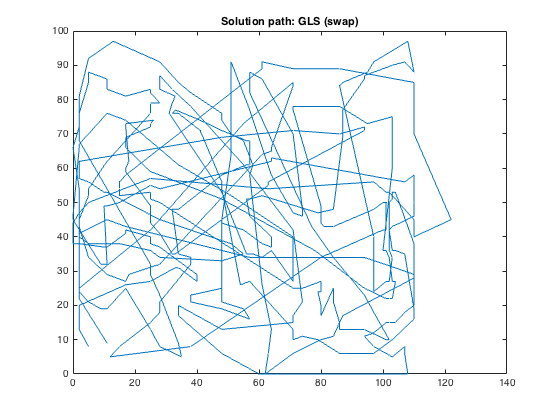
\includegraphics[width=0.7\linewidth]{GLS(swap)}
    \end{subfigure}
    \caption{Improvement Heuristics (Swap)}    
\label{fig:SwapPath}
\end{figure*}

\begin{figure*}[!h]
    \makebox[\textwidth][c]{
    \begin{subfigure}[]{0.7\textwidth}
        \centering
        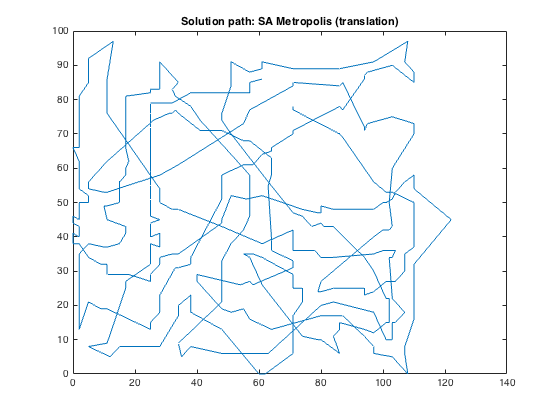
\includegraphics[width=\linewidth]{SAMetropolis(translation)}
    \end{subfigure}
    \begin{subfigure}[]{0.7\textwidth}
        \centering
        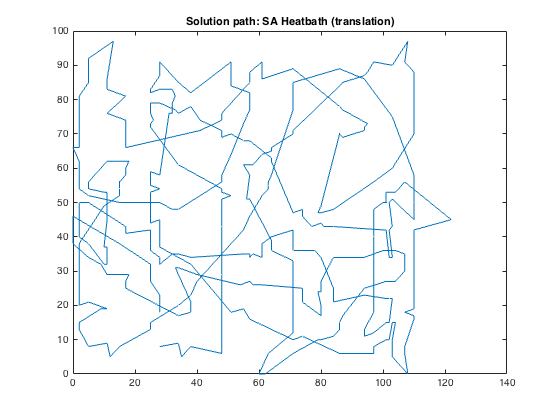
\includegraphics[width=\linewidth]{SAHeatbath(translation)}
    \end{subfigure}
    }
    \begin{subfigure}[]{\textwidth}
        \centering
        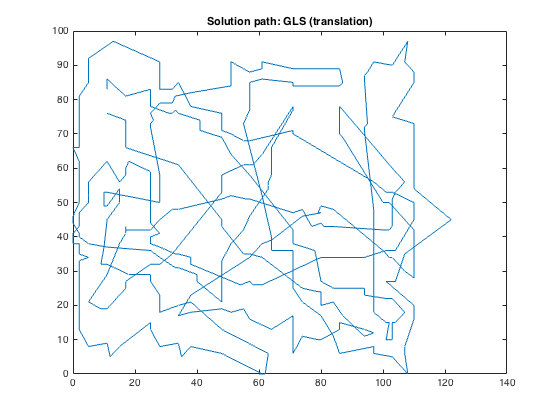
\includegraphics[width=0.7\linewidth]{GLS(translation)}
    \end{subfigure}
    \caption{Improvement Heuristics (Translation)}    
\label{fig:TranslationPath}
\end{figure*}

\begin{figure*}[!h]
    \makebox[\textwidth][c]{
    \begin{subfigure}[]{0.7\textwidth}
        \centering
        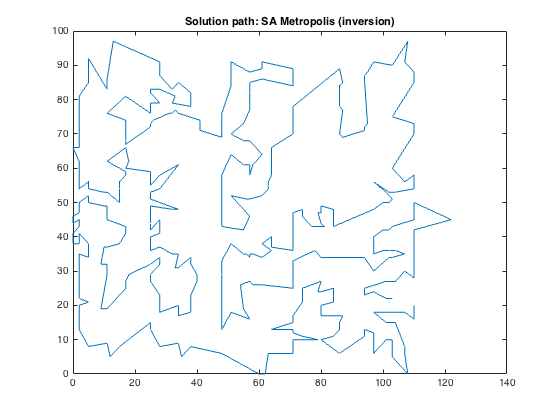
\includegraphics[width=\linewidth]{SAMetropolis(inversion)}
    \end{subfigure}
    \begin{subfigure}[]{0.7\textwidth}
        \centering
        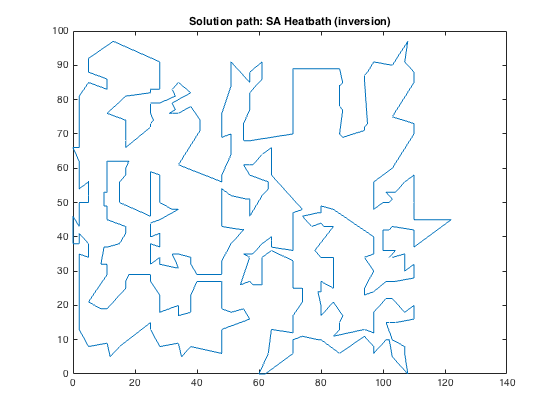
\includegraphics[width=\linewidth]{SAHeatbath(inversion)}
    \end{subfigure}
    }
    \begin{subfigure}[]{\textwidth}
        \centering
        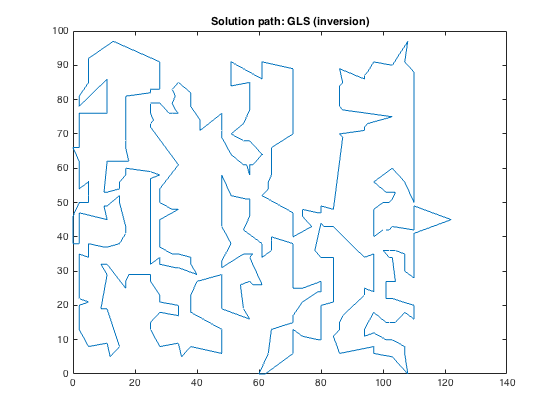
\includegraphics[width=0.7\linewidth]{GLS(inversion)}
    \end{subfigure}
    \caption{Improvement Heuristics (Inversion)}    
\label{fig:InversionPath}
\end{figure*}

\begin{figure*}[!h]
    \makebox[\textwidth][c]{
    \begin{subfigure}[]{0.7\textwidth}
        \centering
        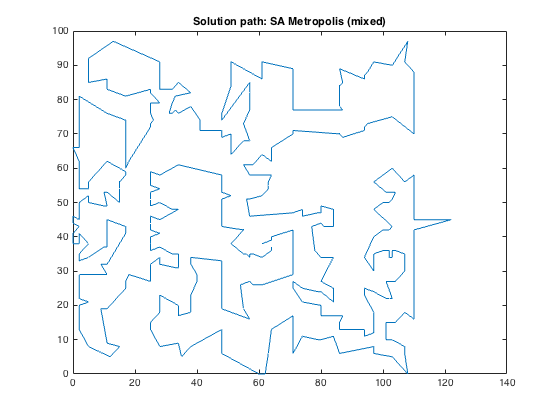
\includegraphics[width=\linewidth]{SAMetropolis(mixed)}
    \end{subfigure}
    \begin{subfigure}[]{0.7\textwidth}
        \centering
        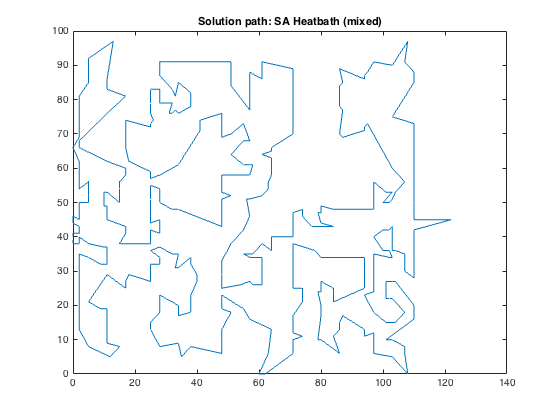
\includegraphics[width=\linewidth]{SAHeatbath(mixed)}
    \end{subfigure}
    }
    \begin{subfigure}[]{\textwidth}
        \centering
        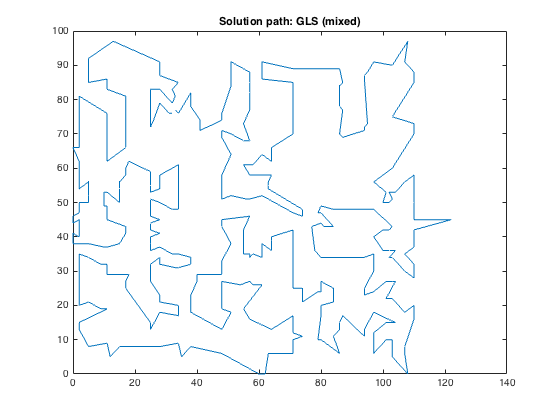
\includegraphics[width=0.7\linewidth]{GLS(mixed)}
    \end{subfigure}
    \caption{Improvement Heuristics (Mixed)}    
\label{fig:MixedPath}
\end{figure*}

\paragraph{3. Performance Plots}
In this section we provide performance plots for the Greedy Local Search (GLS) and Simulated Annealing (SA) algorithms. 

Figures \ref{fig:MetroPerf} and \ref{fig:HBPerf} show the performance-plots for both variants of the SA algorithm. They are based on a single run and show the min, max and mean loss value vs. the current temperature.

The performance-plots for GLS are based on $m=40$ runs and show the min, max and mean loss value against the number of performed moves (Figure \ref{fig:GLSPerf}).

\begin{figure*}[!h]
    \makebox[\textwidth][c]{
 	\begin{subfigure}[]{0.7\linewidth}
        		\centering
        		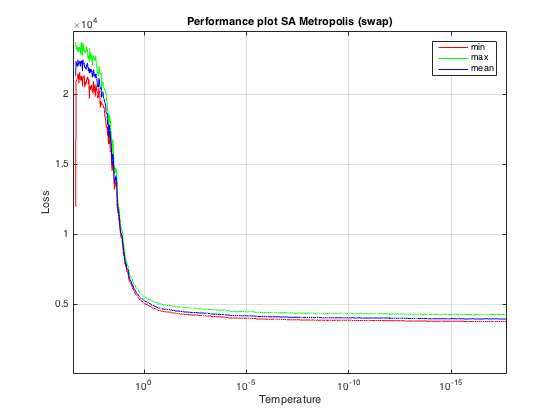
\includegraphics[width=\linewidth]{SAMetropolis(swap)_performance}
    	\end{subfigure}%
    	\begin{subfigure}[]{0.7\linewidth}
		\centering
        		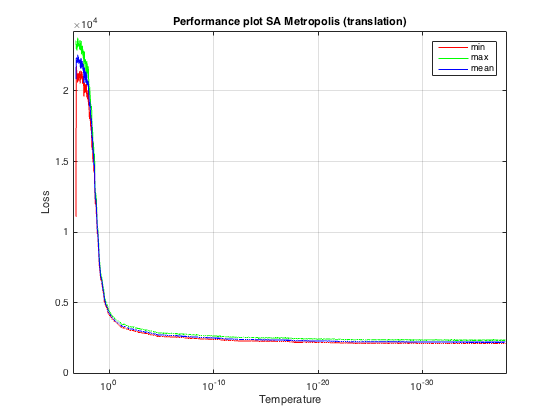
\includegraphics[width=\linewidth]{SAMetropolis(translation)_performance}
    	\end{subfigure}
    }
    \makebox[\textwidth][c]{
 	\begin{subfigure}[]{0.7\linewidth}
        		\centering
        		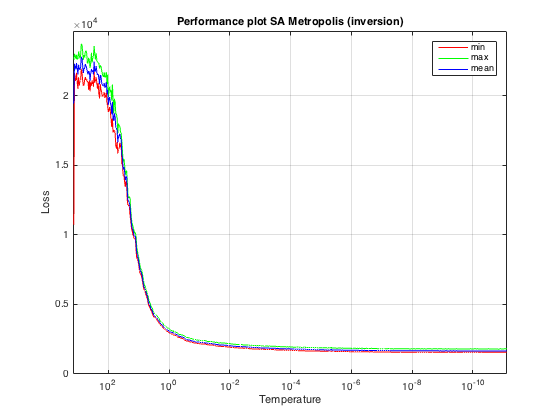
\includegraphics[width=\linewidth]{SAMetropolis(inversion)_performance}
    	\end{subfigure}%
    	\begin{subfigure}[]{0.7\linewidth}
		\centering
        		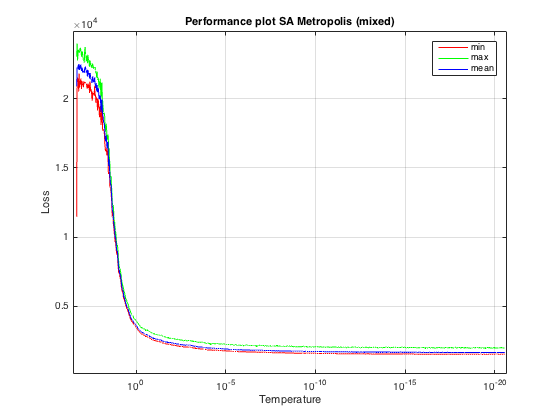
\includegraphics[width=\linewidth]{SAMetropolis(mixed)_performance}
    	\end{subfigure}
    }
    \caption{Performance plots: Simulated Annealing Metropolis}    
\label{fig:MetroPerf}
\end{figure*}

\begin{figure*}[!h]
    \makebox[\textwidth][c]{
 	\begin{subfigure}[]{0.7\linewidth}
        		\centering
        		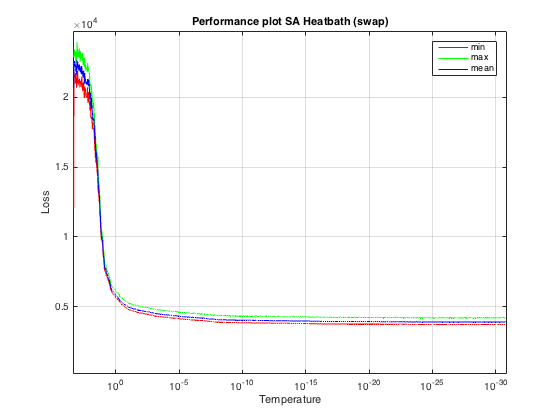
\includegraphics[width=\linewidth]{SAHeatbath(swap)_performance}
    	\end{subfigure}%
    	\begin{subfigure}[]{0.7\linewidth}
		\centering
        		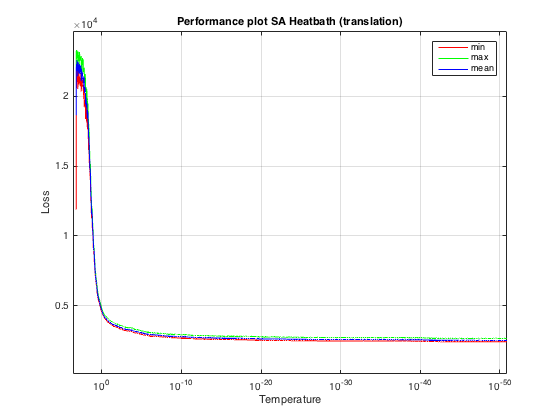
\includegraphics[width=\linewidth]{SAHeatbath(translation)_performance}
    	\end{subfigure}
    }
    \makebox[\textwidth][c]{
 	\begin{subfigure}[]{0.7\linewidth}
        		\centering
        		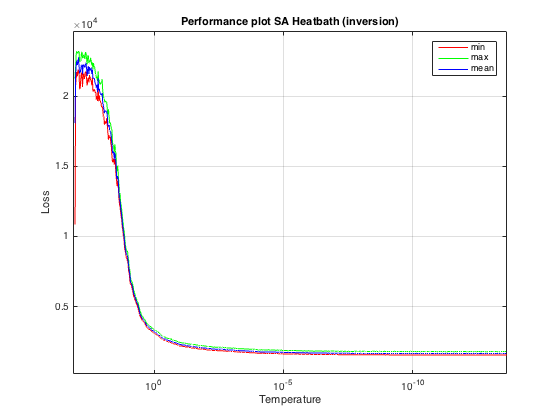
\includegraphics[width=\linewidth]{SAHeatbath(inversion)_performance}
    	\end{subfigure}%
    	\begin{subfigure}[]{0.7\linewidth}
		\centering
        		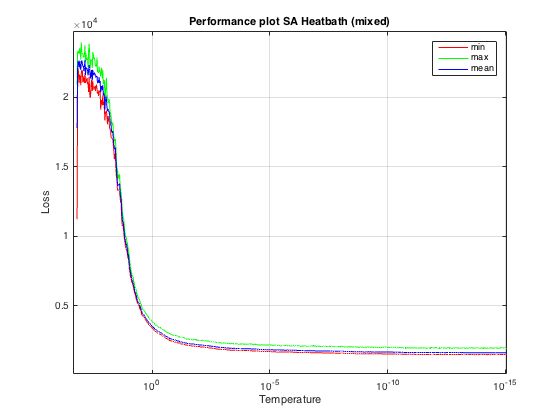
\includegraphics[width=\linewidth]{SAHeatbath(mixed)_performance}
    	\end{subfigure}
    }
    \caption{Performance plots: Simulated Annealing Heatbath}    
\label{fig:HBPerf}
\end{figure*}

\begin{figure*}[!h]
    \makebox[\textwidth][c]{
 	\begin{subfigure}[]{0.7\linewidth}
        		\centering
        		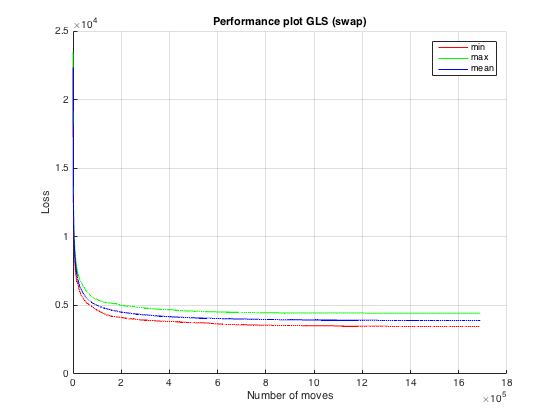
\includegraphics[width=\linewidth]{GLS(swap)_performance}
    	\end{subfigure}%
    	\begin{subfigure}[]{0.7\linewidth}
		\centering
        		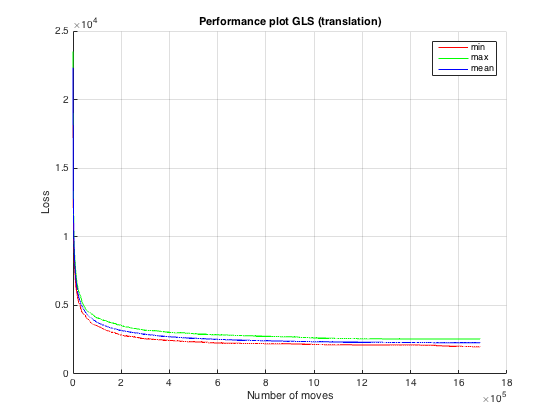
\includegraphics[width=\linewidth]{GLS(translation)_performance}
    	\end{subfigure}
    }
    \makebox[\textwidth][c]{
 	\begin{subfigure}[]{0.7\linewidth}
        		\centering
        		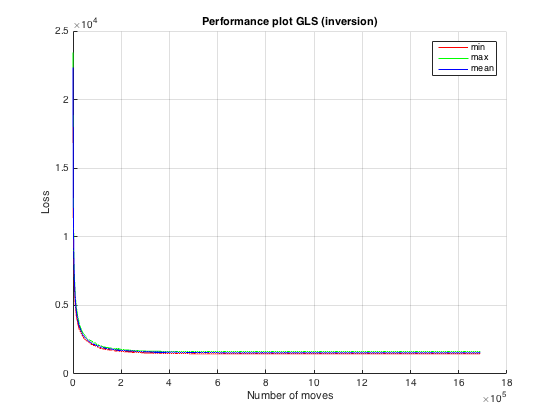
\includegraphics[width=\linewidth]{GLS(inversion)_performance}
    	\end{subfigure}%
    	\begin{subfigure}[]{0.7\linewidth}
		\centering
        		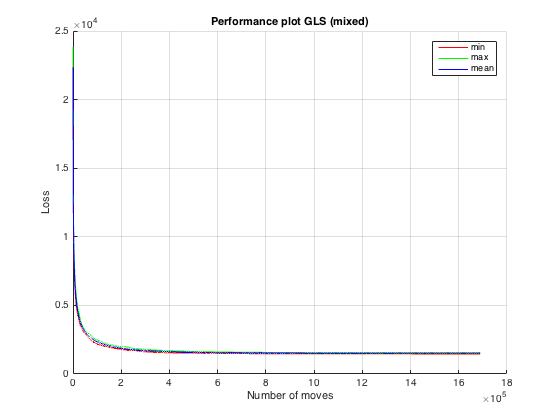
\includegraphics[width=\linewidth]{GLS(mixed)_performance}
    	\end{subfigure}
    }
    \caption{Performance plots: Greedy Local Search}    
\label{fig:GLSPerf}
\end{figure*}

\paragraph{4. Pairwise Comparisons}
Finally in this section the results of the pairwise comparisons of some of the algorithms are shown in table \ref{tab:pairComp}. The comparison was done using an unmatched pair-test with different variances for the two sequences of $m=40$ samples per algorithm.

\begin{table}[!h]
\centering
\caption{Pairwise-Comparison}
\label{tab:pairComp}
\makebox[\textwidth][c]{
\begin{tabular}{|c|c|c|c|c|c|c|}
\hline
Algorithm $A$                  &  Algorithm $B$ & $\mu_A$ & $\mu_B$  & $T$ & $\beta$ & Conclusion \\ \hline \hline
Best Insertion   &   Shortest Edge   &      1.5245    &      1.6725     & -24.4798 &   1.2922  &  $\mu_A < \mu_B$  \\  \hline 
Saving              &   Shortest Edge   &      1.8636    &      1.6725     &  16.9157 &   1.2978  &  $\mu_A > \mu_B$  \\  \hline 
SA Metropolis   &   SA Heatbath     &      1.5155    &      1.5192     &  -0.6661  &   1.2923  &  $\mu_A \approx \mu_B$  \\  \hline 
GLS (swap)      &   GLS (translation)&      3.8952    &      2.2730     &  47.2782  &   1.2935  &  $\mu_A > \mu_B$  \\  \hline 
GLS (swap)      &   GLS (inversion)&      3.8952    &      1.5512     &  82.3048  &   1.3025  &  $\mu_A > \mu_B$  \\  \hline 
GLS (swap)      &   GLS (mixed     )&      3.8952    &      1.5055     &  84.3213  &   1.3029  &  $\mu_A > \mu_B$  \\  \hline 
GLS (translation) &   GLS (inversion)&      2.2730    &      1.5512     &  35.7527  &   1.3014  &  $\mu_A > \mu_B$  \\  \hline 
GLS (translation) &   GLS (mixed)&      2.2730    &      1.5055     &  38.3922  &   1.3022  &  $\mu_A > \mu_B$  \\  \hline 
GLS (inversion) &   GLS (mixed)&      1.5512    &      1.5055     &  7.9280  &   1.2928  &  $\mu_A > \mu_B$  \\  \hline 
\end{tabular}
}
\end{table}

\paragraph{Discussion}

Looking at the results we see that SA and GLS with mixed moves perform the best (achieving the lowest mean-loss), closely followed by the Best-Insertion construction heuristic. 

We can also observe that SA does not considerably perform better or worse than the simple greedy GLS in the given example. Also, the cooling-schedule does not seem to affect the performance of SA in this setting.

The biggest change performance can be observed when comparing the different moves performed. Clearly, Inversion is the most powerful move of the three and combining all of them only provides a minor performance boost (increasing the explorable neighbourhood even more).

 \end{document}